\chapter{Gravitational Fields}
\begin{figure}[H]
    \centering
    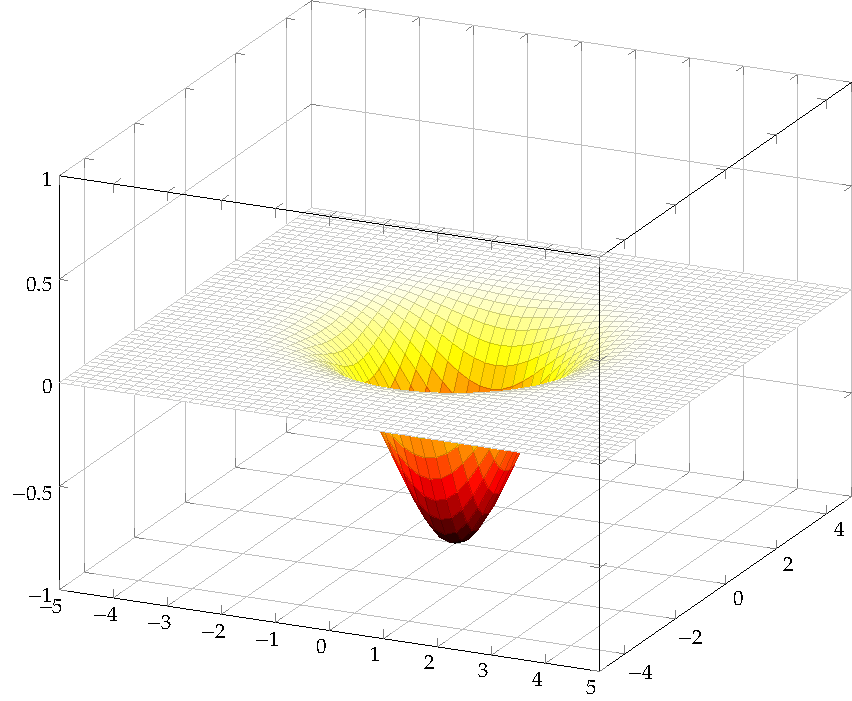
\includegraphics{../images/gravitational-potential-well/gravitational-potential-well-illustration.pdf}
    \caption{\ref{source:gravitational-potential-well} A gravitational potential well.}
    \label{fig:gravitational-potential-well}
\end{figure}
\begin{figure}[H]
    \centering
    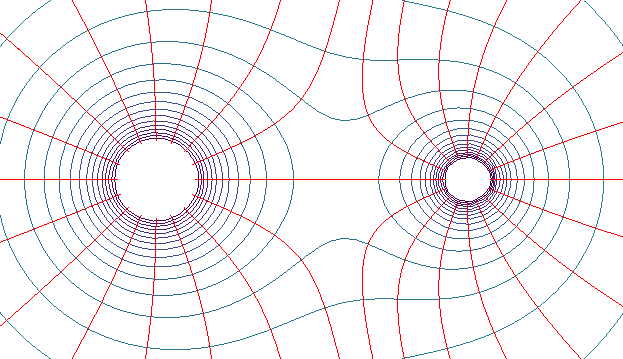
\includegraphics[scale=1.1]{../images/Gravitational-fields-illustration.pdf}
    \caption{\ref{source:G-field-equipotential-lines} The gravitational field and equipotential lines produced by two masses.}
    \label{fig:G-field-equipotential-lines}
\end{figure}
\begin{figure}[H]
    \centering
    \begin{subfigure}{0.45\textwidth}
        \centering
        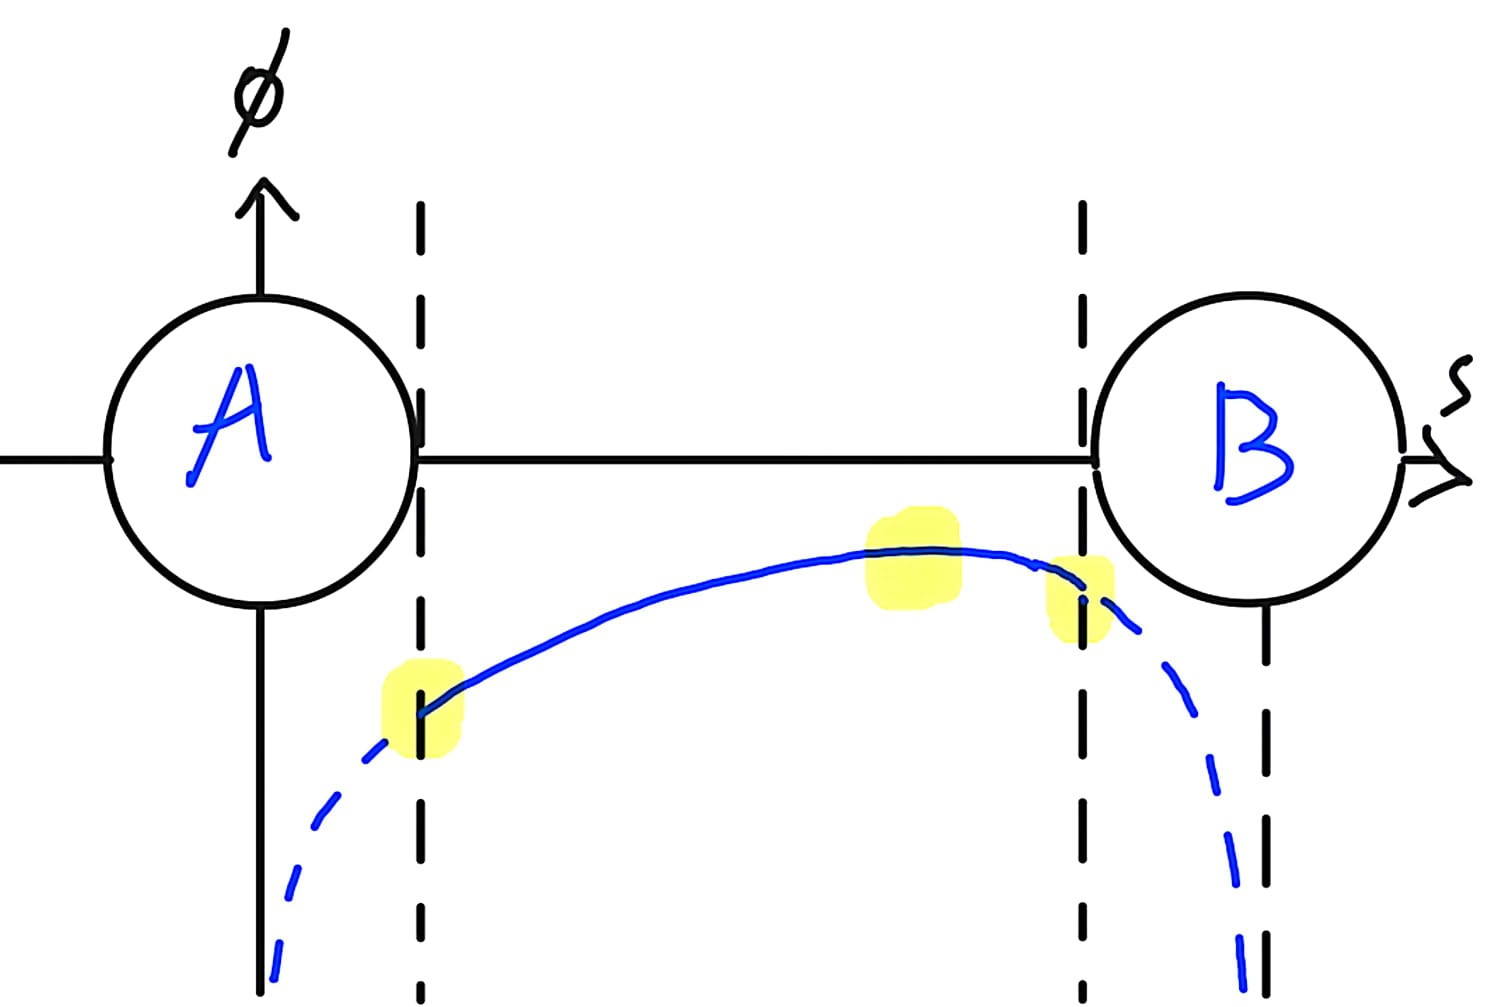
\includegraphics[width=\textwidth]{../images/Two-body-gravity/Potential.jpg}
        \caption{Potential}
        \label{fig:gravitational-potential}
    \end{subfigure}\hfill
    \begin{subfigure}{0.45\textwidth}
        \centering
        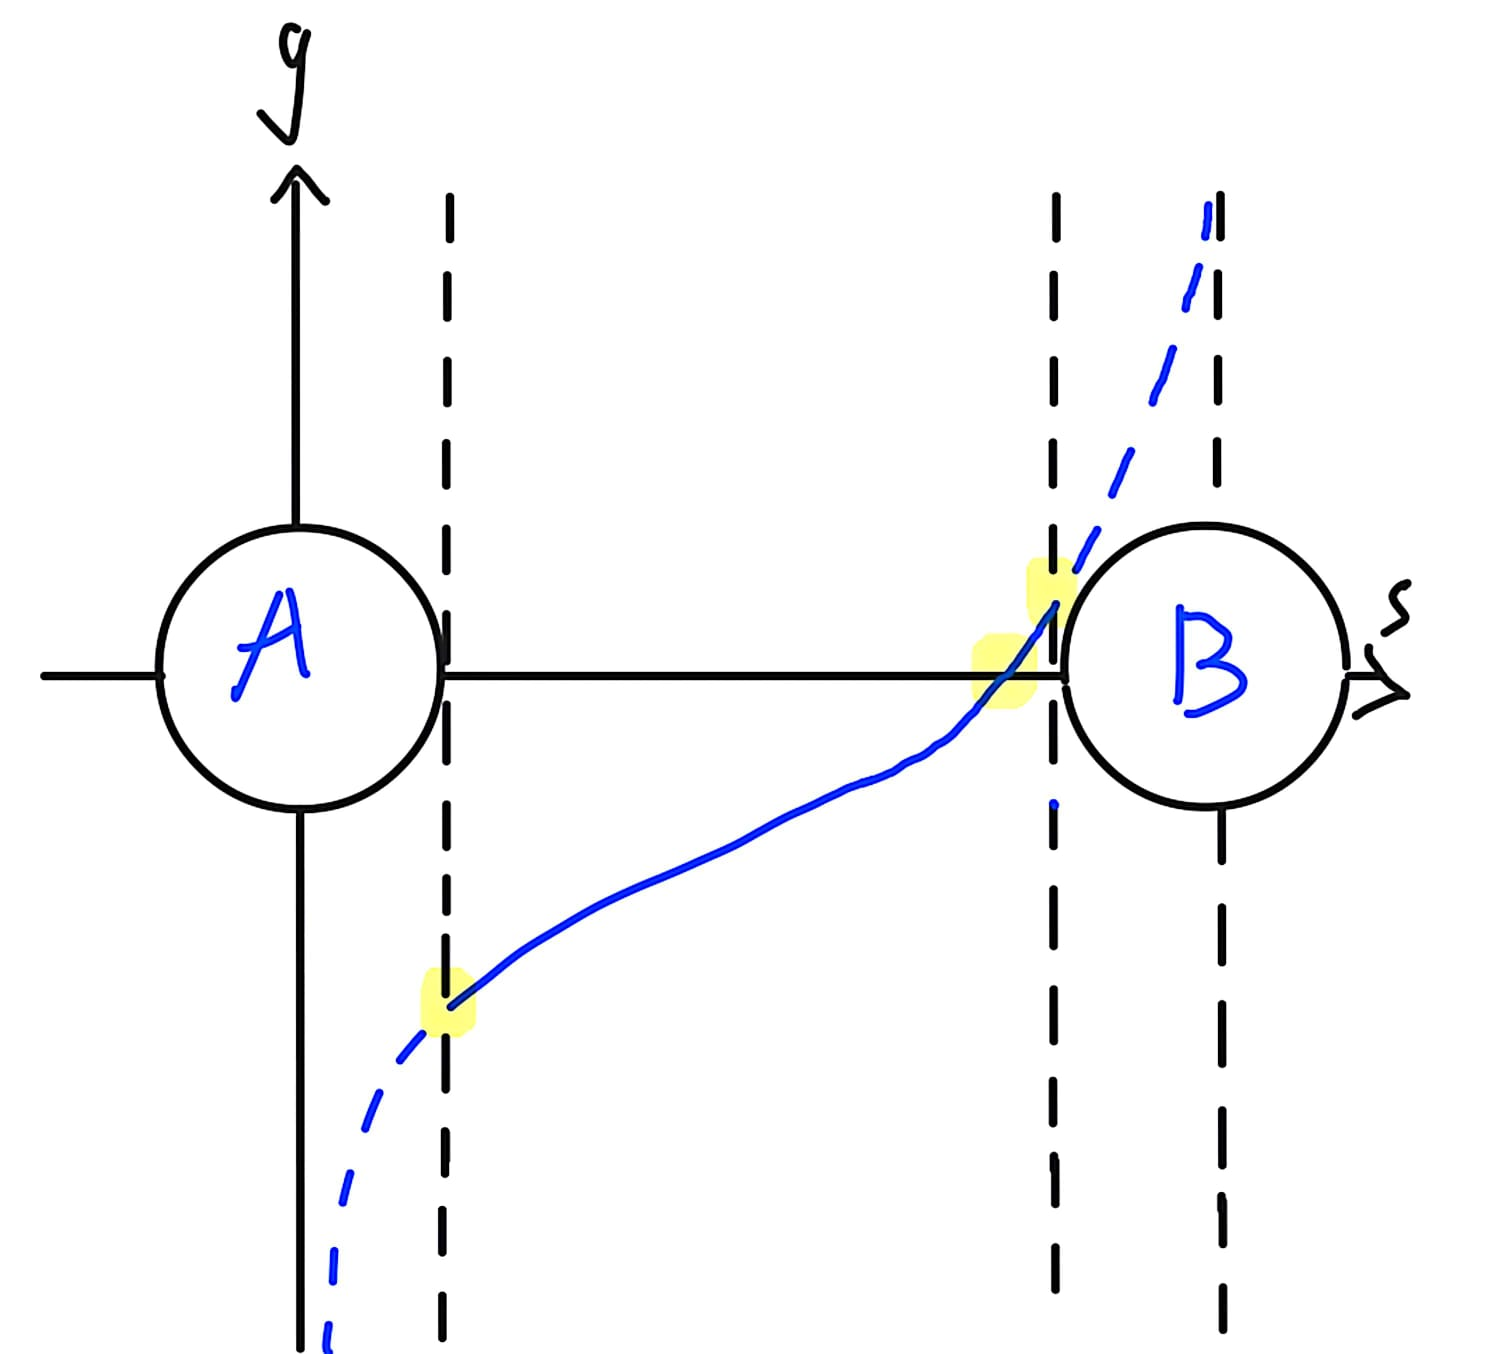
\includegraphics[width=\textwidth]{../images/Two-body-gravity/Field strength.jpg}
        \caption{Field strength}
        \label{fig:gravitational-field-strength}
    \end{subfigure}
    \caption{The gravitational potential and gravitational field strength between two masses.}
    \label{fig:two-body-gravity}
\end{figure}
\begin{itemize}
    \item \emph{Newton's Law of Gravitation} states that the force of attraction between any two point masses is directly proportional to the product of their masses and inversely proportional to the square of their separation.
    \item A \emph{gravitational field} is a region in space where mass experiences a gravitational force acting on it.
    \item Gravitational field strength at a point is defined as the gravitational force per unit mass acting on a small mass placed at that point
    \item The \emph{gravitational potential energy} of a mass at a point is defined as the work done by an \emph{external agent} in bringing the mass \emph{from infinity} to that point (without any net change in kinetic energy).
    \item \emph{Gravitational potential} at a point is defined as the work done per unit mass by an \emph{external agent} in bringing a mass \emph{from infinity} to that point (without a net change in kinetic energy).
    \begin{example}{}{}
        The gravitational potential \(\phi\) at a distance \(x\) from a point mass \(M\) is given by the expression
        \[\phi=-\frac{GM}{x}\]
        where \(G\) is the gravitational constant. Explain why gravitational potential is a negative quantity \hspace*{\fill} [3]
        \begin{itemize}
            \item Since gravitational potential energy is \emph{attractive}, \hspace*{\fill} [1]
            \item an external force that brings a (small test) mass from infinity to a finite distance \(x\) from \(M\), with no net change in kinetic energy, is \emph{opposite in direction} to the displacement of the mass. So, \emph{negative work} is done by the external force. \hspace*{\fill} [1]   
            \item As \emph{gravitational potential at infinity is zero}, the gravitational potential at distance \(x\) from \(M\) is negative. \hspace*{\fill} [1]
        \end{itemize}
    \end{example}
    \item Escape velocity is the \emph{minimum} velocity a mass needs to be projected from the \emph{surface} of the Earth in order to have sufficient kinetic energy to overcome the gravitational field it experiences and \emph{move to infinity}.
    \item Escape velocity \(v_\text{min}=\sqrt{\frac{2GM}{r}}\) (where Min \(E_k\) needed is the gain in \(E_p\) to reach infinity).
\end{itemize}
\begin{itemize}[label=\(\square\)]
    \item \[
\begin{tikzcd}[row sep=large, column sep=large]
     U_G=-\frac{GMm}{r} \arrow{r}{-\frac{\text{d}}{\text{d}r}} \arrow[swap]{d}{\frac{1}{m}} & F_G=-\frac{GMm}{r^2} \arrow[swap]{d}{\frac{1}{m}} \\
     \phi=-\frac{GM}{r} \arrow{r}{-\frac{\text{d}}{\text{d}r}} & g=-\frac{GM}{r^2}
\end{tikzcd}
\]
\item \(U_G=m\phi\) \& \(\Delta U_G=m\Delta\phi\).
% \item \(U_G\) is negative because infinity is taken as the reference point for zero potential energy. The work done against gravitational force in bringing a mass from infinity to that point is negative.
\item Gravitational force provides the centripetal force:
\begin{align*}
    F_G&=F_C\\
    \frac{GMm}{r^2}&=\frac{mv^2}{r}\\
    E_k&=\frac{GMm}{2r}
\end{align*}
Thus, \(E_T=U_G+E_K=-\frac{GMm}{2r}\).
\item Gravitational force provides the centripetal force:
\begin{align*}
    F_G&=F_c\\
    \frac{GMm}{r^2}&=mr\omega^2=mr\left(\frac{2\pi}{T}\right)^2\\
    T^2&=\frac{4\pi^2}{GM}r^3\\
    T^2 &\propto r^3
\end{align*}
\item Gravitational force provides the centripetal force:
\begin{alignat*}{2}
    && F_G&=F_c\\
    &\text{For \(A\):}& \hspace{1cm} \frac{Gm_Am_B}{(r_A+r_B)^2}&=m_Ar_A\omega^2\\
    &\text{For \(B\):}& \frac{Gm_Am_B}{(r_A+r_B)^2}&=m_Br_B\omega^2
\end{alignat*}
The center of mass of the system is at point \(P\) where 
\[m_Ar_A=m_Br_B\]
such that both stars have the same angular velocity \(\omega\).
\item For binary star systems, notice that \emph{orbital radius is replaced by the stars' separation}:
\begin{align*}
    m_Ar_A&=m_Br_B& && \frac{Gm_Am_B}{(r_A+r_B)^2}&=m_Br_B\omega^2\\
    r_A+r_B&=\frac{m_B}{m_A}r_B+r_B& &\text{so}& &=\frac{m_Am_B}{m_A+m_B}(r_A+r_B)\omega^2\\
    r_B&=\frac{m_A}{m_A+m_B}(r_A+r_B)& && &\\
\end{align*}
So, rearranging, we have
\[\omega^2=\frac{G(m_A+m_B)}{(r_A+r_B)^3}=\frac{Gm_A}{r_B(r_A+r_B)^2} \qquad\text{and}\qquad T^2=\frac{4\pi^2}{G(m_A+m_B)}(r_A+r_B)^3.\]
\begin{example}{}{}
    A binary star system has the plane of its orbits parallel to the line of sight from Earth. This binary star system is so far from Earth that the individual stars cannot be distinguished. Suggest and explain what observation can be made to determine the period of the orbit of the stars.
    \begin{itemize}
        \item Observe the light intensity of the binary star system across time.
        \item The minimum intensity occurs when the line joining both stars is parallel to the line of sight from Earth --- one star is directly in front or behind the other so the maximum amount of light from the star behind is blocked by the star in front. 
        \item Determine the time \(t\) between two minimum intensities, which is half a period. The orbital period is \(T=2t\). 
    \end{itemize}
\end{example}
\item Geostationary orbit facts:
\begin{enumerate}
    \item Only one such orbit at a \emph{fixed} distance of \(4.2\times10^7\text{m}\) from Earth's center,
    \item Orbital period of 24 hours,
    \item Satellite's plane of orbit coincides with the equatorial plane of the Earth,
    \item Orbits West to East (in the same direction as Earth's rotation). 
\end{enumerate}
\item Equipotential lines are not equally spaced because gravitational field strength is not constant but decreases as one goes away from the Earth.
\item Assumptions made in the theory (e.g. in deriving \(g=-\frac{GM}{r^2}\)):
\begin{enumerate}
    \item The bodies are separated by distances so large they can be considered as point particles (i.e. separation >> radius).
    \item The bodies are homogenous spheres (constant density throughout the sphere).
    \item The bodies have masses distributed symmetrically around their centers in uniform layers.
    \item In the absence of other masses.
\end{enumerate}
\begin{example}{}{}
    State and explain the effect, if any, on the graph --- of gravitational field strength against the distance from the center of the sphere --- you have sketched on Fig 9.2 when mass is lost uniformly from the surface of the sphere. \hspace*{\fill} [2]
    \begin{itemize}
        \item The gravitational field strength \(g\) still obeys the inverse square law. But since \(g\) is directly proportional to the mass of the sphere, \(g\) decreases. \hspace*{\fill} [1]
        \item Hence, the new graph will be shifted down and entirely below the original graph. \hspace*{\fill} [1]
    \end{itemize}
\end{example}
\end{itemize}
\begin{center}
    \includegraphics[width=\textwidth]{../images/2024-Eclipse-Map-(cit\_).png}
    \captionsetup{type=figure}
    \caption[figure]{\ref{2024 Eclipse Map} Forces acting on a crane.}
\end{center}
\emph{Note.} According to the author of this image, when compared to their above prediction,
\begin{enumerate}
    \item The duration of eclipse at greatest eclipse is 2 seconds shorter.
    \item The moments of contact are a couple seconds off.
\end{enumerate}